\section{Overall System Evaluation}

\subsection{Experiment Setup}
This experiment will be deducted at the student Firas house, since it is very suitable because it contains multiple floors, and filed with obstacles, representing the average indoor environments.

The building manager - which in this experiment is Firas - will need to log the QR codes into the dashboard(or create new account of he does not already have one. See figure \ref{overall_system_experiment_SigUp}) and links them in the proper way. See figure \ref{overall_system_experiment_Manage} that show the real process of logging one of the QR codes. And see figure \ref{overall_system_experiment_Linking} which illustrates the linking process.

\begin{figure}[h!]
	\centering
	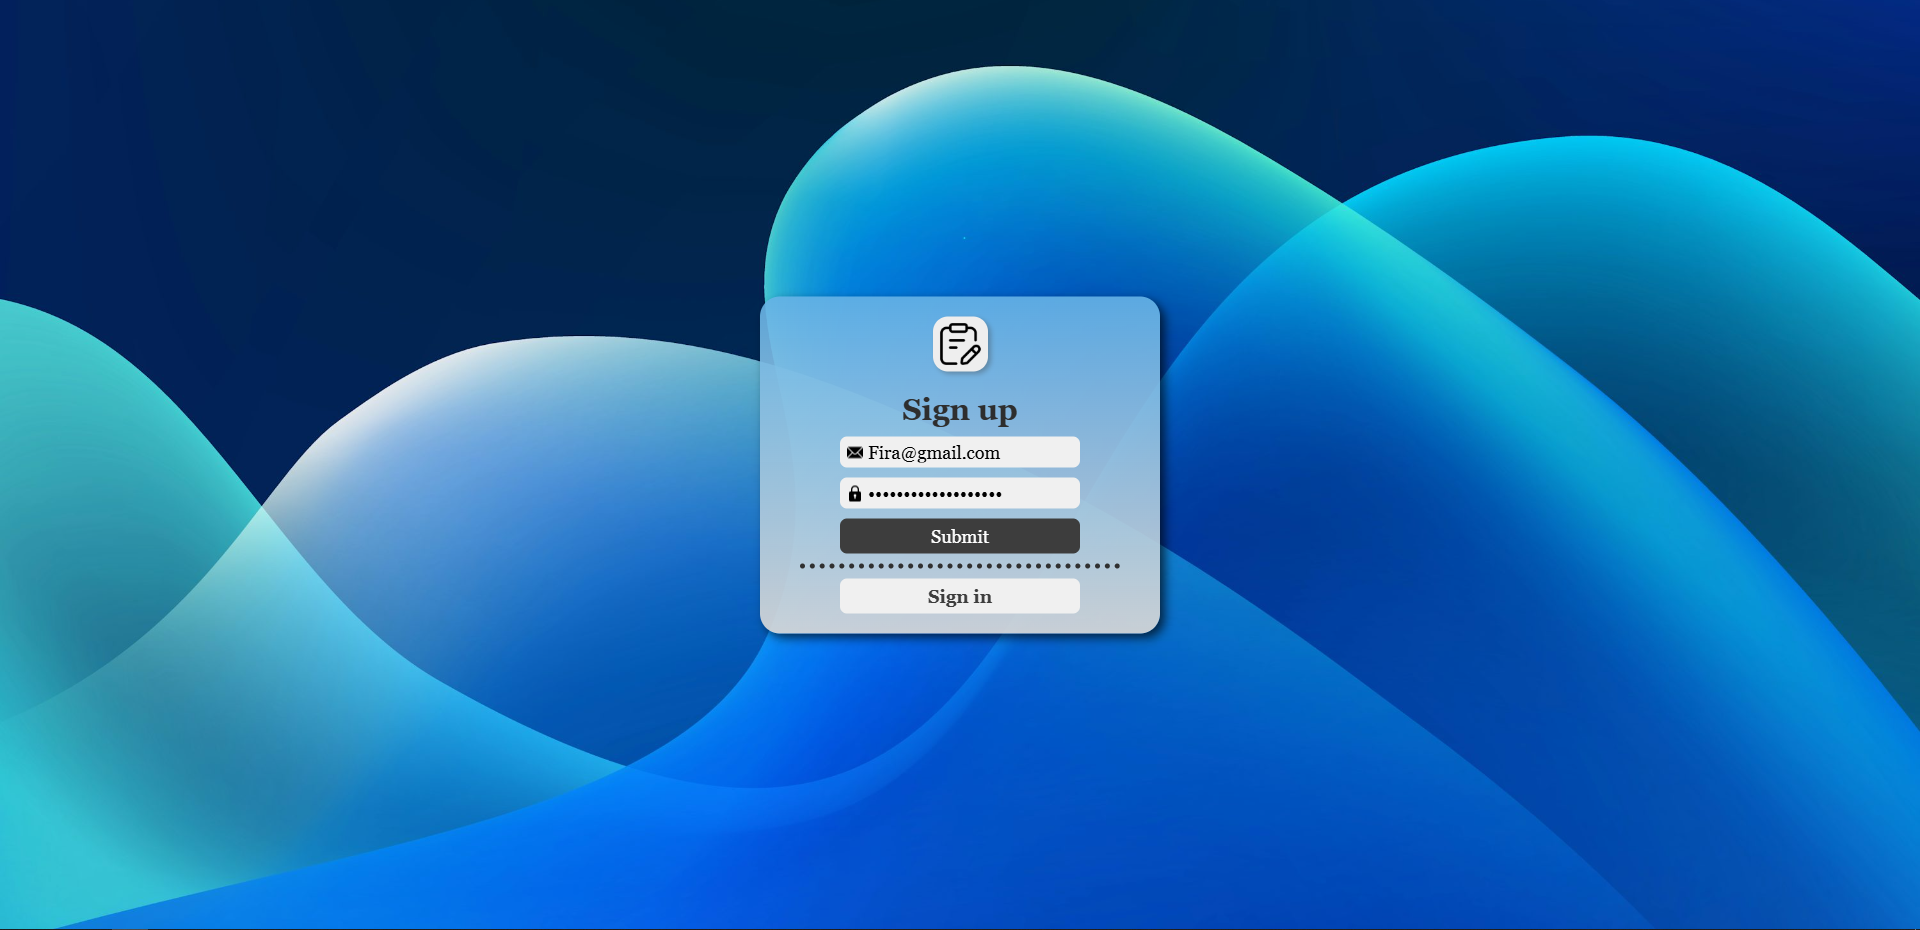
\includegraphics[width=0.7\linewidth]{assets/Overrall System Experiment/Sign Up.png}
	\caption{This screenshot shows the sign up page at the dashboard.}
	\label{overall_system_experiment_SigUp}
\end{figure}

\begin{figure}[h!]
	\centering
	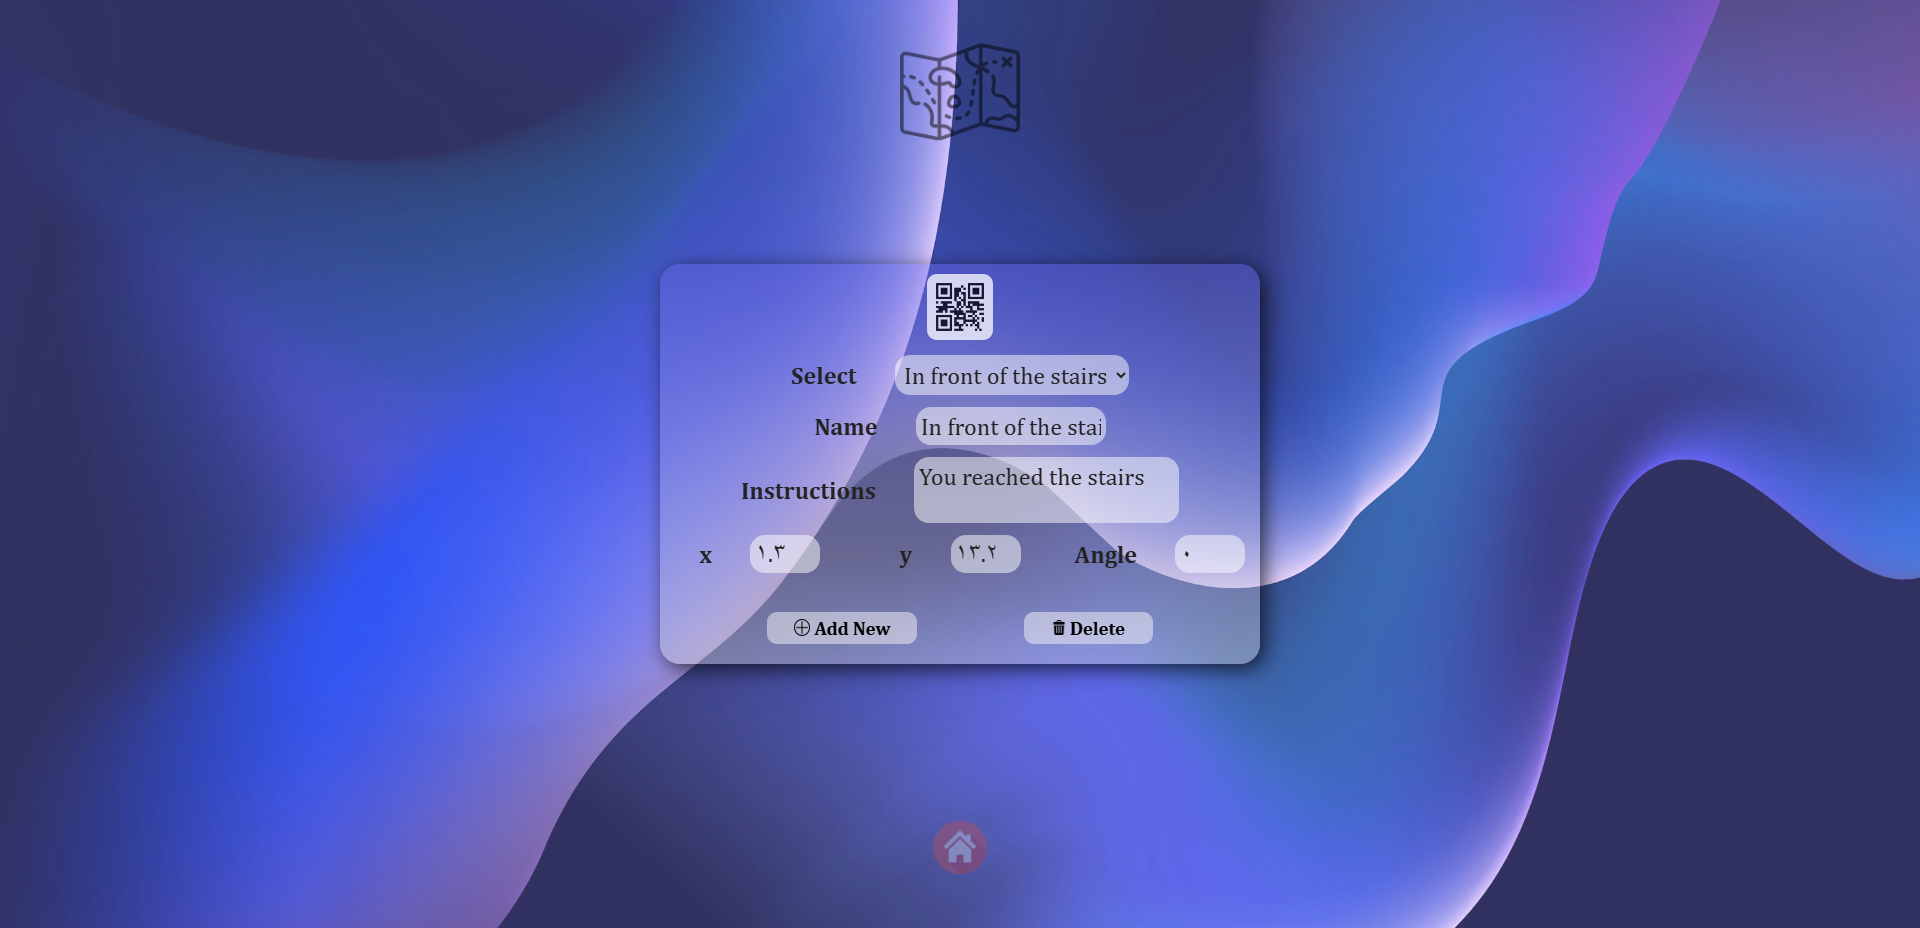
\includegraphics[width=0.7\linewidth]{assets/Overrall System Experiment/Manage.png}
	\caption{This screenshot shows the data logging page at the dashboard.}
	\label{overall_system_experiment_Manage}
\end{figure}

\begin{figure}[h!]
	\centering
	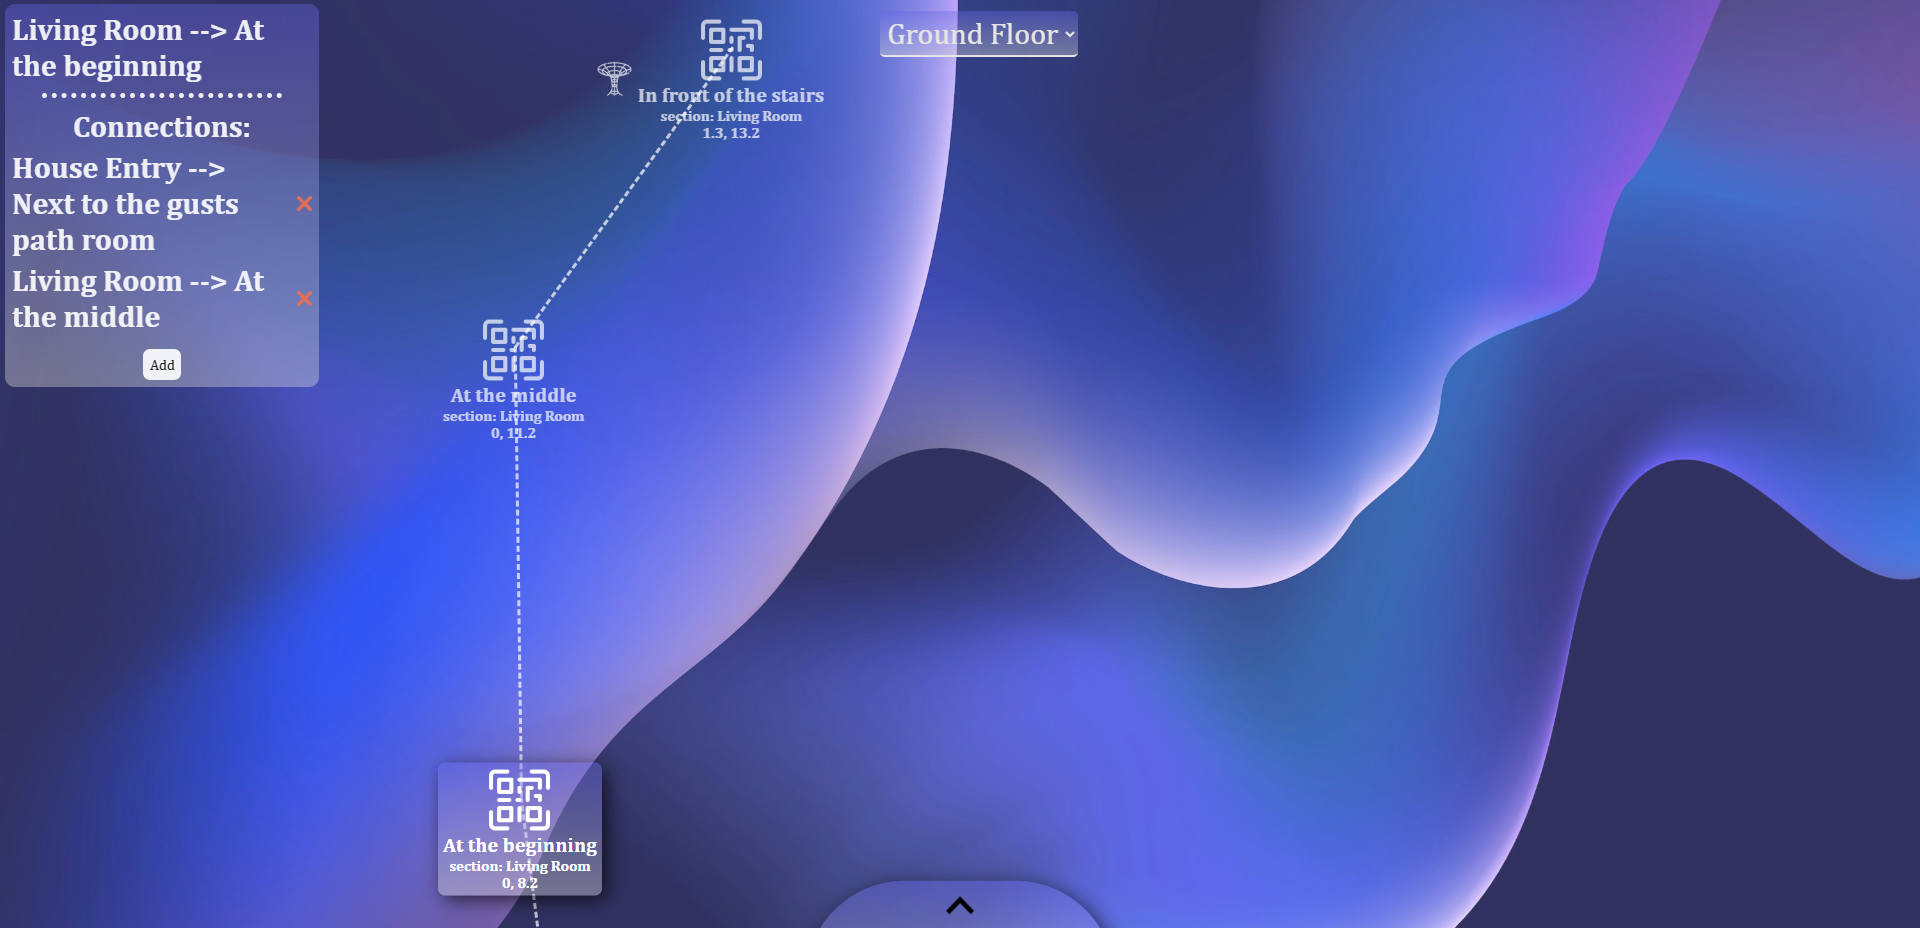
\includegraphics[width=0.7\linewidth]{assets/Overrall System Experiment/Linking.png}
	\caption{This screenshot shows the linking page at the dashboard.}
	\label{overall_system_experiment_Linking}
\end{figure}

See figures \ref{overall_system_experiment_Ground_Floor_Structure}. and \ref{overall_system_experiment_First_Floor_Structure} to understand the structure of the used floors and the QR codes places.

\begin{figure}[h!]
	\centering
	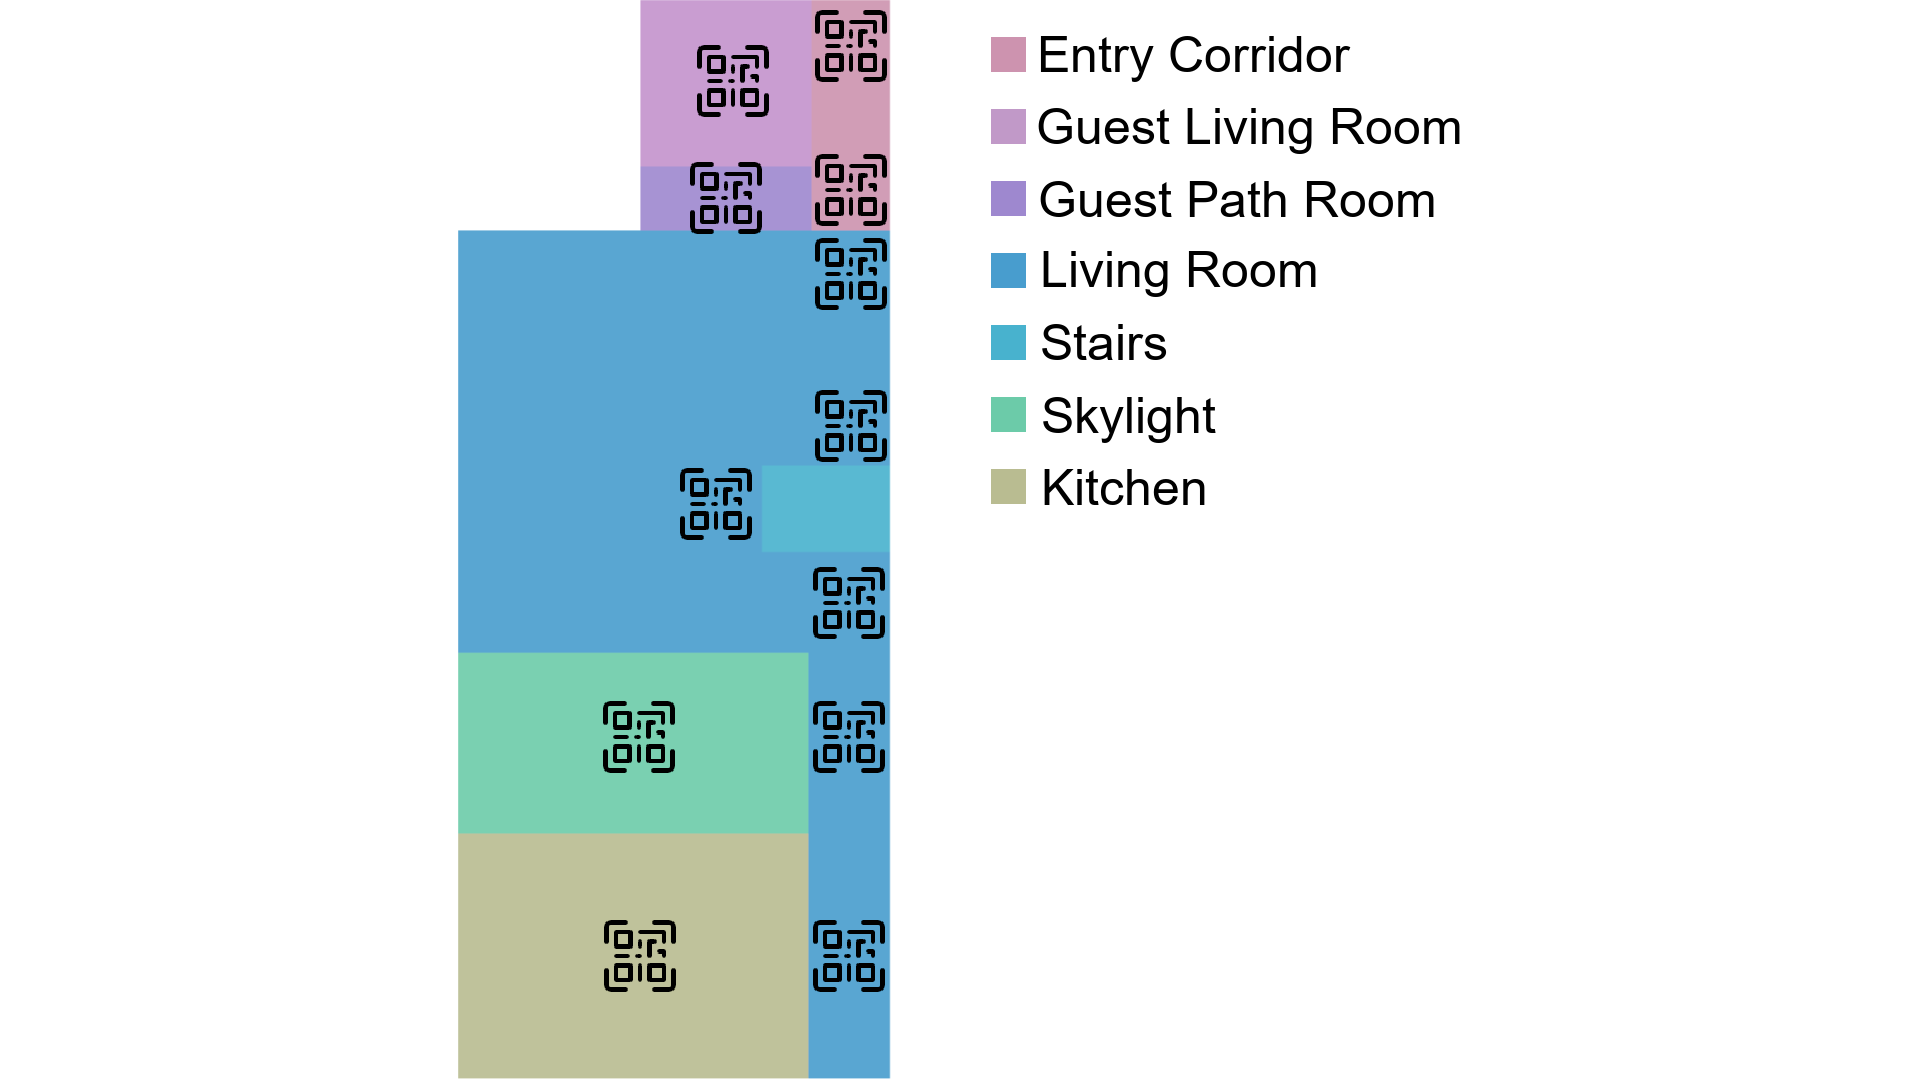
\includegraphics[width=0.7\linewidth]{assets/Overrall System Experiment/Ground Floor Structure.png}
	\caption{This figure illustrates the structure of the ground floor. The QR codes are put only in the necessary areas for the system to work properly.}
	\label{overall_system_experiment_Ground_Floor_Structure}
\end{figure}

\begin{figure}[h!]
	\centering
	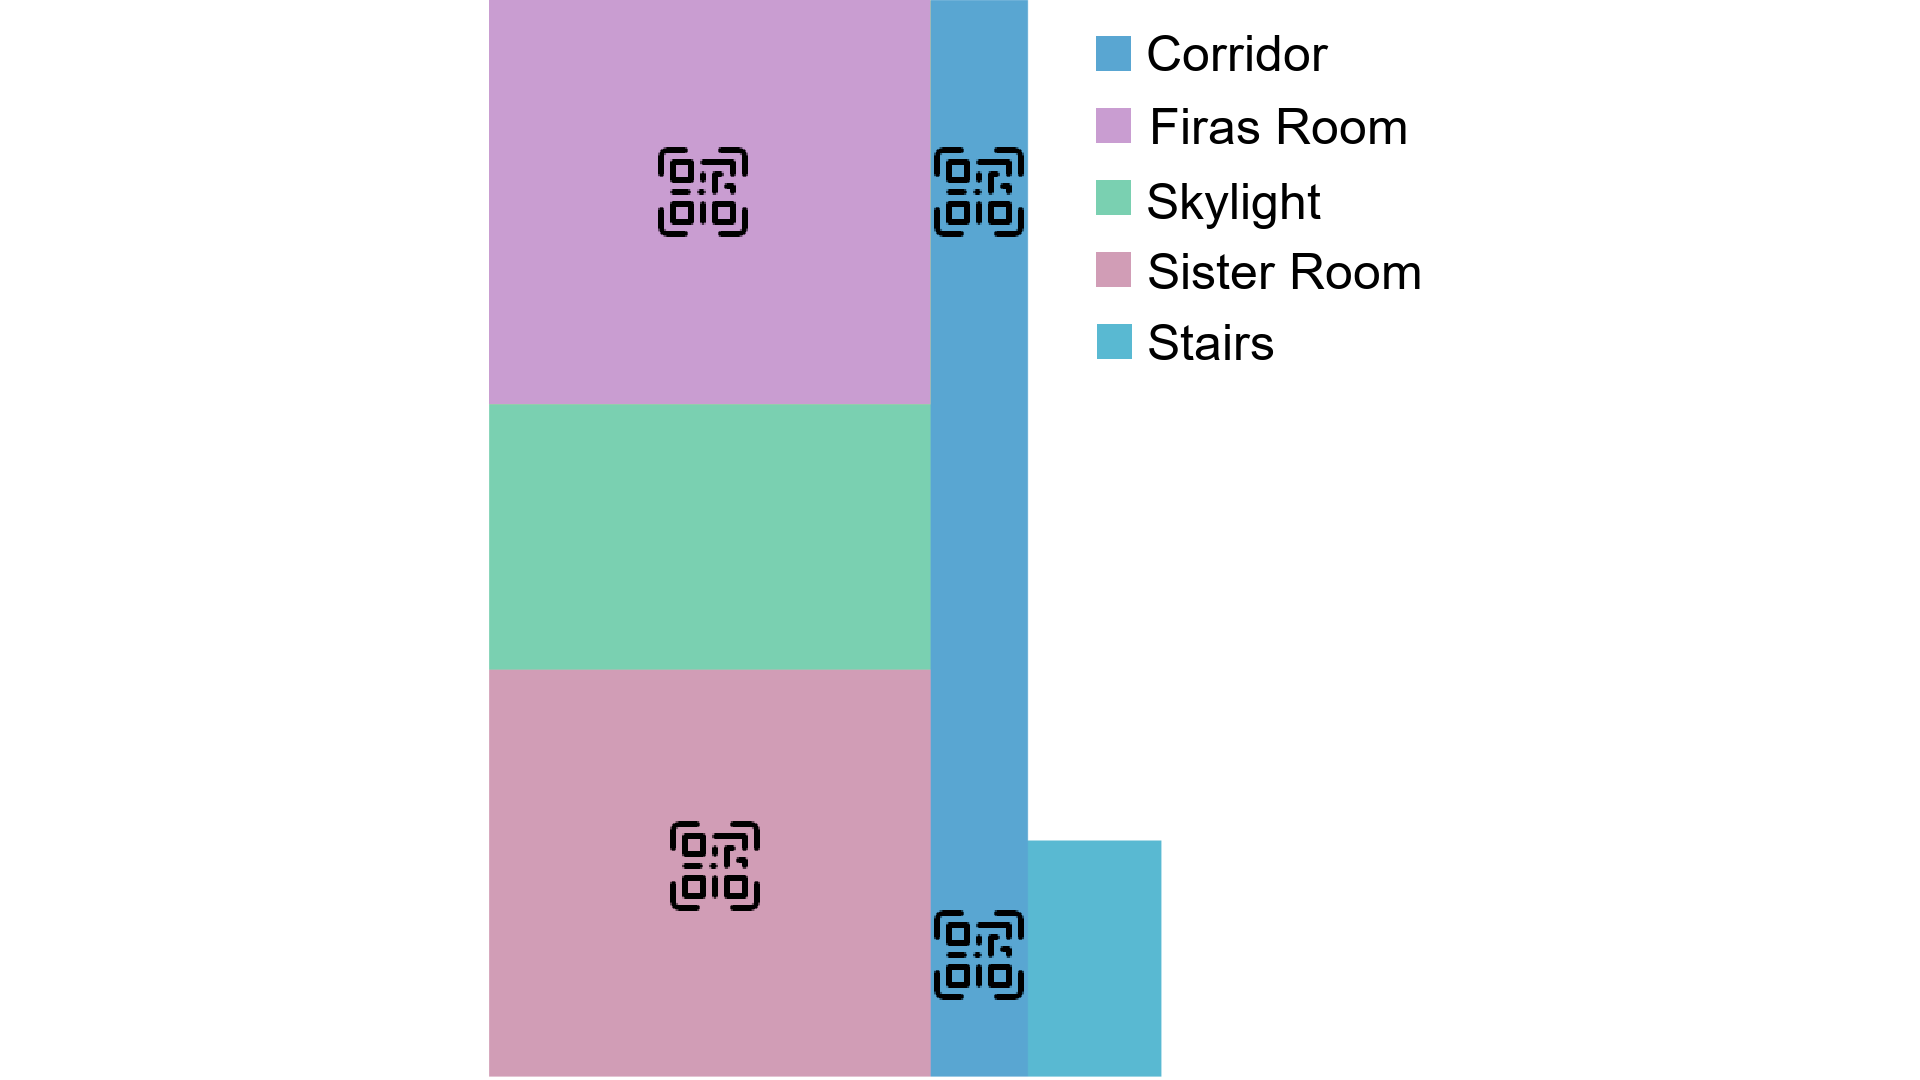
\includegraphics[width=0.7\linewidth]{assets/Overrall System Experiment/First Floor Structure.png}
	\caption{This figure illustrates the structure of the first floor. The QR codes are put only in the necessary areas for the system to work properly.}
	\label{overall_system_experiment_First_Floor_Structure}
\end{figure}

\subsection{Procedure}
The starts by the user being standing at the souse entry at the ground floor, then the system will guide him/her to the selected destination. In this experiment, the user want to go to Firas room at the first floor.

The system must read instructions to the user informing him/her about the surrounding sections, and it also must guide the user reaching to the selected destination.

At each milestone, the system must provide guidance and informative instructions as it described at \ref{Customizable Guidance Methodology Section}. All instructions for a specific milestone will be logged along with the user current location to ease following the experiment progress.

Finally, the experiment must end after the user being at the selected destination by, and only by, following the system instructions.

\subsection{Evaluation Metrics}
The evaluation metrics applied in this study are described in detail in Section~\ref{sec:evaluation_metrics} of the Methodology chapter. All results and analyses presented here are based on those metrics.


\subsection{Results}
\textbf{Milestone 1:}\\
\textbf{Instructions:}\\
This is the house of Firas Ghazi AlSadiq. You are welcome here.\\
\color{green}Then after 1.5s:\color{black}\\
This is the ground floor. It contains the gusts room, the gusts path room, the living room, and the kitchen.\\
\color{green}Then after 1.5s:\color{black}\\
This is the entry of the house. From here, you will be able to access the gusts room, the gusts path room, and the living room.\\
\textbf{Guidance:}\\
Walk 5.5 meters\\
\textbf{Milestone position:} (0, 0)\\
\\
\textbf{Milestone 2:}\\
\textbf{Instructions:}\\
\textbf{Guidance:}\\
Walk 2.7 meters\\
\textbf{Milestone position:} (0, 5.5)\\
\\
\textbf{Milestone 3:}\\
\textbf{Instructions:}\\
This is the living room. It is connected with the house entry, and the kitchen.\\
\textbf{Guidance:}\\
Walk 3 meters\\
\textbf{Milestone position:} (0, 8.2)\\
\\
\textbf{Milestone 4:}\\
\textbf{Instructions:}\\
\textbf{Guidance:}\\
Walk 2.4 meters at 33\textdegree to the right\\
\textbf{Milestone position:} (0, 11.2)\\
\\
\textbf{Milestone 5:}\\
\textbf{Instructions:}\\
\textbf{Guidance:}\\
You reached the stairs\\
\textbf{Milestone position:} (1.3, 13.2)\\
\\
\textbf{Milestone 6:}\\
\textbf{Instructions:}\\
This is the first floor. It contains Firas room, his path room, his sister room, and her path room.\\
\color{green}Then after 1.5s:\color{black}\\
This is a corridor that leads to Firas room, and his sister room.\\
\textbf{Guidance:}\\
Walk 4 meters\\
\textbf{Milestone position:} (0, 0)\\
\\
\textbf{Milestone 7:}\\
\textbf{Instructions:}\\
\textbf{Guidance:}\\
Walk 1.5 meters at 90\textdegree to the left\\
\textbf{Milestone position:} (0, 4)\\
\\
\textbf{Milestone 8:}\\
\textbf{Instructions:}\\
This is Firas room which is connected to Firas path room, and to the corridor.\\
\textbf{Guidance:}\\
You reached your destination\\
\textbf{Milestone position:} (-1.5, 4)\\

\subsection{Results Discussion}
The system managed to inform the user by all the sections important information and provided the needed guidance to the selected destination.